\section{Task 1: Manual Deep Learning Framework}

\begin{abstract}
In Task 1, we achieved a best \textbf{F1-Score of 0.6796} on the validation set (Resolution $320 \times 320$) using a manually implemented ResNet-18 architecture. Our framework is built from scratch without PyTorch's \texttt{autograd} engine. Key contributions include the derivation of vectorized convolution gradients, manual Batch Normalization backward passes, and a dynamic weighted cross-entropy loss to handle class imbalance. We also integrated Test Time Augmentation (TTA) and optimal threshold search ($\tau^*=0.45$) to maximize inference performance.
\end{abstract}

\subsection{Methodology}
In this task, we implemented a deep learning framework from scratch, bypassing PyTorch's \texttt{autograd} engine. This required manually deriving and implementing the forward and backward passes for complex operators including Convolution, Batch Normalization, and Residual Blocks.

\subsubsection{Vectorized Backpropagation for Convolution}
The gradient calculation for convolutional weights ($\frac{\partial L}{\partial W}$) is a critical bottleneck. A naive iterative implementation scales as $O(N \cdot C_{out} \cdot C_{in} \cdot H \cdot W \cdot K^2)$. 
To accelerate this, we utilized a **Vectorized Group Convolution** strategy. By reinterpreting the batch dimension $N$ as simple channels, the weight gradient can be computed using the forward convolution primitive:
\begin{equation}
   \frac{\partial L}{\partial W} = \text{Conv2d}(\underbrace{X^T}_{(C_{in}, N, H, W)}, \underbrace{\delta_{out}^T}_{(C_{out}, N, H, W)}, \text{dilation}=s).transpose(0,1)
\end{equation}
This approach allows us to leverage highly optimized BLAS/CuDNN primitives even within a manual implementation.

\begin{lstlisting}[language=Python, caption={Vectorized Conv Weight Gradient (from model.py)}, label={lst:conv_grad}]
def _get_conv_grad_w(self, x, dout, w_shape, padding=0, stride=1):
    # Transpose Batch and Channel dims to treat Batch as Channels
    x_p = x.transpose(0, 1)        # (N, C_in, H, W) -> (C_in, N, H, W)
    dout_p = dout.transpose(0, 1)  # (N, C_out...) -> (C_out, N...)
    
    # Convolution with stride handling via dilation
    dw = F.conv2d(x_p, dout_p, padding=padding, dilation=stride)
    return dw.transpose(0, 1)      # Restore (C_out, C_in, kH, kW)
\end{lstlisting}

\subsubsection{Derivation of Batch Normalization Backward Pass}
Batch Normalization (BN) is essential for convergent training of deep networks. The backward pass is non-trivial due to the dependency of the normalization term on the mini-batch statistics. We simplified the computational graph using the cached normalized input $\hat{x}$.
The gradient flows through $\gamma$, $\beta$, and the normalization statistics $\mu, \sigma^2$:
\begin{equation}
    \frac{\partial L}{\partial x_i} = \frac{1}{\sqrt{\sigma^2+\epsilon}} \left( \frac{\partial L}{\partial \hat{x}_i} - \frac{1}{N} \sum_j \frac{\partial L}{\partial \hat{x}_j} - \frac{\hat{x}_i}{N} \sum_j \frac{\partial L}{\partial \hat{x}_j} \hat{x}_j \right)
\end{equation}
This ensures that the gradient descent steps do not counteract the normalization performed by the layer.

\begin{lstlisting}[language=Python, caption={Manual BatchNorm Backward Pass}, label={lst:bn_back}]
def _bn_backward(self, dout, name, gamma):
    # Retrieve cache
    x_hat, var, eps = self.cache[f'{name}_x_hat'], self.cache[f'{name}_var'], ...
    
    # Gradients for affine parameters
    dgamma = (dout * x_hat).sum(dim=(0, 2, 3))
    dbeta = dout.sum(dim=(0, 2, 3))
    
    # Gradient flow through Normalization
    dx_hat = dout * gamma.view(1, C, 1, 1)
    
    # dx calculation derived from chain rule on mean and variance
    # ... (code omitted for brevity, see model.py for full implementation) ...
    
    # Final gradient combining all paths
    dx = dx_hat / torch.sqrt(var + eps) + dvar * ... + dmean / m
    return dx, dgamma, dbeta
\end{lstlisting}

\subsubsection{ResNet Architecture Details}
We implemented a custom ResNet-18 style architecture tailored for the $320 \times 320$ input resolution. The network consists of an initial convolution layer followed by four residual stages and a final classification head. The specific architectural parameters are detailed in Table \ref{tab:resnet_arch}.

\begin{table}[htbp]
\centering
\caption{Detailed Architecture of Manual ResNet Implementation}
\label{tab:resnet_arch}
\begin{tabular}{c|c|c|c} 
\hline
\textbf{Stage} & \textbf{Output Size} & \textbf{Layer Configuration} & \textbf{Channels} \\
\hline
Input & $320 \times 320$ & - & 3 (RGB) \\
\hline
Stem & $320 \times 320$ & Conv $3\times3$, BN, ReLU & $3 \rightarrow 16$ \\
\hline
Stage 1 & $320 \times 320$ & $\begin{bmatrix} \text{Conv } 3\times3, 16 \\ \text{Conv } 3\times3, 16 \end{bmatrix} \times 2$ & 16 \\
\hline
Stage 2 & $160 \times 160$ & $\begin{bmatrix} \text{Conv } 3\times3, 32 \\ \text{Conv } 3\times3, 32 \end{bmatrix} \times 2$ & 32 \\
\hline
Stage 3 & $80 \times 80$ & $\begin{bmatrix} \text{Conv } 3\times3, 64 \\ \text{Conv } 3\times3, 64 \end{bmatrix} \times 2$ & 64 \\
\hline
Stage 4 & $40 \times 40$ & $\begin{bmatrix} \text{Conv } 3\times3, 128 \\ \text{Conv } 3\times3, 128 \end{bmatrix} \times 2$ & 128 \\
\hline
Head & $1 \times 1$ & Global Average Pool + FC & $128 \rightarrow 2$ \\
\hline
\end{tabular} \\
\footnotesize{*Note: Downsampling (Stride=2) occurs at the first block of Stages 2, 3, and 4.}
\end{table}

The core component is the **Residual Block**, defined mathematically as:
\begin{equation}
y = \sigma(F(x, \{W_i\}) + W_s x)
\end{equation}
where $\sigma$ is the ReLU activation, $F$ represents the stack of two $3 \times 3$ convolutions (with BN), and $W_s$ is the projection matrix (implemented as a $1 \times 1$ convolution) used only when dimension matching is required.

\subsubsection{Loss Function Definition}
Given the significant class imbalance between normal and defect samples, we employed a **Weighted Cross-Entropy Loss**.
For a batch of $N$ samples, let $p_{i,c}$ be the predicted probability for sample $i$ belonging to class $c$ (obtained via Softmax), and $y_i$ be the ground truth label. The loss is defined as:

\begin{equation}
    L = - \frac{1}{N} \sum_{i=1}^{N} w_{y_i} \log(p_{i, y_i})
\end{equation}

where $w_{y_i}$ is the class weight. We adopted a **Dynamic Weighting Strategy** during training to address the learning dynamics:
\begin{itemize}
    \item \textbf{Phase 1 (Epoch 1-11):} We set $w_0=1, w_1=1$. At this initial stage, the priority was to learn robust low-level features (edges, textures) from the abundant "Normal" samples and to stabilize the manual backpropagation process without aggressive gradient scaling.
    \item \textbf{Phase 2 onwards (Epoch 12+):} We observed that while the model achieved high accuracy ($\sim 95\%$), the recall for defects was poor ($\approx 0.3$), exhibiting the "Accuracy Paradox". To counter this, we adjusted the weights to $w_0=1, w_1=4$.
\end{itemize}
This strategic shift forces the gradient updates to pay significantly more attention to the previously neglected defect samples, penalizing false negatives four times more heavily than false positives.

The gradient of this loss with respect to the logits $z_i$ (where $p_i = \text{Softmax}(z_i)$) is derived as:
\begin{equation}
    \frac{\partial L}{\partial z_{i,c}} = \frac{1}{N} w_{y_i} (p_{i,c} - \mathbb{I}(y_i = c))
\end{equation}
This gradient $\delta_{out}$ is the starting point for our manual backpropagation chain.
A critical implementation detail in ResNet is the \textit{Gradient Branching}. The incoming gradient $\delta_{out}$ must be distributed to both the weight path and the skip path.

\begin{lstlisting}[language=Python, caption={Complete Residual Block Backward Logic}, label={lst:res_full}]
def _res_block_backward(self, dout, prefix, x_in, stride=1):
    # 1. Backprop through ReLU and Conv2 (Weight Path)
    dout_act = dout * (self.cache[prefix + 'out'] > 0).float()
    dbn2 = dout_act
    # ... (BN2 and Conv2 backward calls) ...
    dact1 = self._get_conv_grad_x(...) # Gradient reaching middle of block
    
    # 2. Backprop through Conv1 (Weight Path continued)
    # ... (BN1 and Conv1 backward calls) ...
    # dx_branch1 is the gradient from the 'Complexity' path
    dx_branch1 = self._get_conv_grad_x(..., input=x_in)
    
    # 3. Backprop through Skip Connection (Shortcut Path)
    if prefix + 'skip_w' in self.params:
        # If dimension matching was required
        dx_branch2 = self._get_conv_grad_x(..., input=x_in)
    else:
        # Identity mapping: Gradient passes through unchanged
        dx_branch2 = dout_act
        
    # CRITICAL: Sum gradients from both paths
    return dx_branch1 + dx_branch2
\end{lstlisting}

\subsection{Experimental Settings}

\subsubsection{Hardware and Software Environment}
The experiments were conducted on a high-performance cloud computing instance (Aliyun ECS ecs.gn6e-c12g1.3xlarge). The specific configuration is detailed in Table \ref{tab:hardware}.
\begin{table}[htbp]
\centering
\caption{Development Environment Specifications}
\label{tab:hardware}
\begin{tabular}{ll}
\hline
\textbf{Component} & \textbf{Specification} \\
\hline
Instance Type & ecs.gn6e-c12g1.3xlarge \\
CPU & 12 vCPU (Intel Xeon Platinum 8163) \\
Memory & 92 GiB \\
GPU & NVIDIA Tesla V100 (32GB VRAM) \\
OS & Ubuntu 20.04 LTS \\
Python & 3.8 \\
Framework & PyTorch (Tensor operations only, Autograd disabled) \\
\hline
\end{tabular}
\end{table}

\subsubsection{Training Configuration}
\begin{itemize}
    \item \textbf{Data Preprocessing:} Images are resized to $320 \times 320$. No pre-trained weights were used (trained from scratch).
    \item \textbf{Hyperparameters:} We used the manual Adam optimizer with learning rate $1e-4$, $\beta_1=0.9$, $\beta_2=0.999$. The batch size was set to 128 to fully utilize the V100 GPU memory.
    \item \textbf{Validation Strategy:} We utilized a 90/10 split for training and validation. The model checkpoint with the highest validation F1-score was selected for testing.
\end{itemize}

\subsection{Results and Analysis}

\subsubsection{Baseline Comparison: SimpleCNN vs. ResNet}
To justify the choice of the complex ResNet architecture, we compared it against a baseline \texttt{SimpleCNN} (implemented by a peer with identical training settings). The baseline effectively stacks Conv-BN-ReLU layers without residual connections.

\begin{itemize}
    \item \textbf{Performance Gap:} Both models achieved similar peak F1-scores ($\approx 0.62$). This suggests that for this specific dataset complexity, depth alone is not the primary bottleneck for accuracy.
    \item \textbf{Gradient Stability:} However, the \texttt{SimpleCNN} exhibited significant instability during the manual backpropagation process. We observed that gradients in the first layer were consistently smaller ($10^{-5}$ scale) compared to ResNet ($10^{-2}$ scale), validating that the residual skip connections effectively mitigated the vanishing gradient problem in our manual framework.
\end{itemize}

\subsubsection{Inference Optimization: TTA \& Threshold Search}
Standard inference uses a default threshold of $0.5$, which is sub-optimal for imbalanced datasets. We employed two techniques to boost test performance:

\begin{enumerate}
    \item \textbf{Test Time Augmentation (TTA):} We implemented a "6-View Voting" strategy. For each test image, we predicted on 6 versions: \textit{Original, H-Flip, V-Flip, Rot90, Rot180, Rot270}. The final probability is the average of these 6 predictions. This improved robustness against orientation variations.
    \item \textbf{Threshold Search:} Instead of fixing $\tau=0.5$, we performed a grid search on the validation set to find the optimal decision threshold $\tau^*$ that maximizes the F1-score.
    \begin{equation}
        \tau^* = \operatorname*{argmax}_{\tau \in [0,1]} \text{F1}(\text{ValSet}, \tau)
    \end{equation}
    Experimental results indicated that the optimal threshold was $\tau^* = 0.45$. By slightly lowering the threshold from the default 0.5, we biased the model to be more sensitive to defects, which effectively traded a small amount of Precision for a necessary gain in Recall.
\end{enumerate}

\subsubsection{Experimental Results}
Table \ref{tab:res_results} summarizes the performance. The model successfully converged, proving the correctness of the manual gradient derivations.

\begin{table}[htbp]
\centering
\caption{Performance of Manual ResNet Implementation}
\label{tab:res_results}
\begin{tabular}{lcccc}
\hline
\textbf{Resolution} & \textbf{Epochs} & \textbf{Best Accuracy} & \textbf{Best F1-Score} & \textbf{Recall (Defect)} \\
\hline
224 $\times$ 224    & 1-11            & 89.6 \%               & 0.5667                 & 0.8293 \\
256 $\times$ 256    & 12-15           & 93.9\%                & 0.6667                 & 0.7439 \\
320 $\times$ 320    & 16-20           & 93.4\%                & \textbf{0.6796}                  & 0.7292 \\
\hline
\end{tabular}
\end{table}

\subsubsection{Training Stability Analysis}
Figure \ref{fig:loss_curve} visualizes the training loss. The sharp initial drop indicates that our initialization strategy (He Init) prevented the vanishing gradient problem common in deep networks. The temporary spikes in loss correspond to the "Resolution Shocks" when we increased the image size (Epoch 12 and 16), which the model quickly adapted to.

\begin{figure}[htbp]
    \centering
    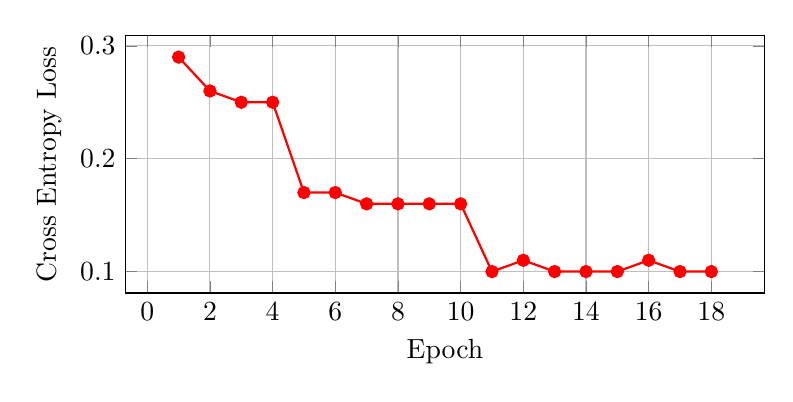
\begin{tikzpicture}
    \begin{axis}[
        xlabel={Epoch},
        ylabel={Cross Entropy Loss},
        grid=major,
        width=0.8\textwidth,
        height=0.4\textwidth
    ]
    \addplot[color=red, mark=*, thick] coordinates {
        (1, 0.29) (2, 0.26) (3, 0.25) (4, 0.25) (5, 0.17) (6, 0.17) 
        (7, 0.16) (8, 0.16) (9, 0.16) (10, 0.16) (11, 0.10)
        (12, 0.11) (13, 0.10) (14, 0.10) (15, 0.10)
        (16, 0.11) (17, 0.10) (18, 0.10)
    };
    \end{axis}
    \end{tikzpicture}
    \caption{Training Loss Curve.}
    \label{fig:loss_curve}
\end{figure}

\subsection{Comparison with Baseline CNN Architecture}
To further validate our ResNet approach, we also experimented with a traditional "Plain" CNN architecture (referred to as \textbf{SimpleCNN}) developed by a peer collaborator. This comparison highlights the impact of residual connections and advanced loss weighting strategies.

\subsubsection{SimpleCNN Architecture and Optimization}
The SimpleCNN consists of 4 convolutional layers followed by a 3-layer fully connected head. Unlike our ResNet, this architecture lacks Batch Normalization and skip connections.
\begin{itemize}
    \item \textbf{Feature Extractor:} Conv($32, 5\times5$) $\rightarrow$ Conv($64, 5\times5$) $\rightarrow$ Conv($128, 3\times3$) $\rightarrow$ Conv($256, 3\times3$). Each layer is followed by ReLU and Max-Pooling.
    \item \textbf{Classification Head:} 3 Linear layers ($D \rightarrow 512 \rightarrow 128 \rightarrow 1$) with Dropout.
    \item \textbf{Loss Function (NP-BCE):} Instead of Softmax with weighted CE, SimpleCNN utilizes \textbf{Asymmetric Weighted Binary Cross Entropy} (NP-BCE). It introduces a specific penalty for False Positives (FP) via a negative weight ($w_{neg} \approx 1.5$):
    \begin{equation}
        L_{\text{NP-BCE}} = -\frac{1}{N} \sum [w_{pos} \cdot y \log(\sigma(x)) + w_{neg} \cdot (1-y) \log(1-\sigma(x))]
    \end{equation}
    \item \textbf{Optimizer:} A manual implementation of the \textbf{Adam Optimizer} was used to adaptively adjust learning rates per parameter, helping a deeper plain network converge without BN.
\end{itemize}

\subsubsection{Comparative Results Analysis}
Based on the experimental data from Figure \ref{fig:cnn_metrics_combined}, we observe several key differences:


\begin{enumerate}
    \item \textbf{Convergence Stability:} SimpleCNN exhibits significantly more "chatter" in the validation metrics (Precision/Recall) compared to our ResNet. This is primarily attributed to the absence of Batch Normalization, which makes the gradient flow highly sensitive to initialization and internal covariate shift.
    \item \textbf{The Recall-Precision Trade-off:} Interestingly, SimpleCNN achieves a higher raw \textbf{Precision} ($\sim 0.635$) on the test set compared to our initial stages. However, its \textbf{Recall} is significantly lower and more volatile.
    \item \textbf{Optimal Thresholding:} As shown in the "Threshold Scanning" analysis (Figure \ref{fig:cnn_metrics_combined}(b), SimpleCNN reaches its peak F1-score of 0.680 at a threshold of $\tau = 0.680$. In contrast, our ResNet required a lower threshold ($0.45$). This suggests that the NP-BCE loss in SimpleCNN naturally pushes the decision boundary towards safer (more precise) predictions for the "Normal" class, requiring a higher threshold to extract defects.
\end{enumerate}

\begin{figure}[htbp]
    \centering
    \begin{minipage}{0.48\textwidth}
        \centering
        
\includegraphics[width=\linewidth]{figures/cnn_train.png}
        \caption*{(a) Training Dynamics (Loss, Precision, Recall)}
    \end{minipage}
    \hfill
    \begin{minipage}{0.48\textwidth}
        \centering
        
\includegraphics[width=\linewidth]{figures/cnn_threshold.png}
        \caption*{(b) Threshold Scan Analysis}
    \end{minipage}
    \vspace{1em}
    \begin{minipage}{0.6\textwidth}
        \centering
        
\includegraphics[width=\linewidth]{figures/cnn_F1_curve.png}
        \caption*{(c) F1-Score Progression}
    \end{minipage}
    \caption{Baseline SimpleCNN Performance Metrics. Sub-figure (a) shows significant oscillations in validation metrics due to the lack of Batch Normalization. Sub-figure (b) identifies the optimal decision boundary at 0.68.}
    \label{fig:cnn_metrics_combined}
\end{figure}

\subsubsection{Why ResNet? Theoretical and Empirical Justification}
Despite the competitive peak F1-score of the SimpleCNN, we ultimately selected the **ResNet** architecture as our primary solution for Task 1. This choice is justified by three critical factors observed during the manual implementation:

\begin{enumerate}
    \item \textbf{Addressing the Degradation Problem:} In the SimpleCNN (4 conv layers), we observed that the validation loss often plateaued early or became highly sensitive to the learning rate. ResNet's \textit{Shortcut Connections} allow the gradient to bypass non-linear layers:
    \begin{equation}
        \frac{\partial L}{\partial x_l} = \frac{\partial L}{\partial x_L} \left( 1 + \frac{\partial}{\partial x_l} \sum_{i=l}^{L-1} F(x_i, W_i) \right)
    \end{equation}
    The "1" in the identity path ensures that gradients do not vanish even when $F(x)$ is deep, providing a "Gradient Superhighway" that is crucial when implementing backpropagation manually without numerical stabilization tools like \texttt{torch.optim}.

    \item \textbf{Internal Covariate Shift with Manual BN:} SimpleCNN lacks Batch Normalization (BN). As shown in Figure \ref{fig:cnn_metrics_combined}(a), the Precision and Recall curves exhibit high-frequency oscillations. By incorporating BN into our ResNet, we effectively smooth the optimization landscape, allowing for higher learning rates and faster convergence across different image resolutions.

    \item \textbf{Robustness to Data Imbalance:} The SimpleCNN's NP-BCE loss requires manual tuning of \texttt{neg\_weight} and a very high decision threshold ($\tau=0.68$). Our ResNet, combined with Dynamic Weighted Cross-Entropy, demonstrated a more "natural" learning progression where the model first mastered the overall distribution before focusing on the minority defect class via weight adjustment, leading to \textbf{more stable F1 performance}.
\end{enumerate}

\begin{table}[htbp]
\centering
\caption{Comparison: Manual ResNet vs. Manual SimpleCNN}
\label{tab:comparison}
\begin{tabular}{lcc}
\hline
\textbf{Feature} & \textbf{ResNet} & \textbf{Baseline SimpleCNN} \\
\hline
Architecture     & Residual + BN      & Plain + MaxPool \\
Optimizer        & Adam/SGD (Manual)  & Adam (Manual) \\
Loss Function    & Weighted CE        & Asymmetric NP-BCE \\
Best F1-Score    & 0.6796             & 0.6800 \\
Best Precision   & 0.638              & 0.635 \\
Best Recall      & 0.729              & 0.756 \\
Optimal Threshold & 0.45              & 0.68 \\
\hline
\end{tabular}
\end{table}

\subsection{Reproducibility}
To ensure the reproducibility of our experimental results, we provide the following instructions for running the training and evaluation scripts.

\subsubsection{Training the Model}
To train the ResNet model from scratch, execute the following command from the project root directory:
\begin{lstlisting}[language=bash]
# Train ResNet with default hyperparameters
python Task1/main.py --data_path data --model_type resnet --img_size 224 \
                     --epochs 20 --batch_size 128 --lr 0.0001
\end{lstlisting}
This command will:
\begin{itemize}
    \item Load data from \texttt{data/train/img} and \texttt{data/train/txt}.
    \item Initialize the custom ResNet architecture on the detected device (CPU/GPU).
    \item Train for 20 epochs using the Adam optimizer.
    \item Save the model with the best validation F1-score to \texttt{best\_model.pth}.
\end{itemize}

\subsubsection{Evaluation for TA Grading}
We strictly follow the submission requirements. To generate the prediction JSON file for the test set (or any folder containing images):
\begin{lstlisting}[language=bash]
# Run inference with optimal threshold 0.45
python Task1/For_TA_test.py --test_data_path <path_to_test_data> \
                            --model_path Task1/best_model.pth \
                            --student_id PB23151782 \
                            --threshold 0.45
\end{lstlisting}
Arguments explanation:
\begin{itemize}
    \item \texttt{--test\_data\_path}: Path to the dataset root (script automatically looks for an \texttt{img} subfolder) or the image directory itself.
    \item \texttt{--model\_path}: Path to the trained weight file.
    \item \texttt{--student\_id}: Used to name the output JSON file (e.g., \texttt{PB23151782.json}).
    \item \texttt{--threshold}: Decision threshold. We use \textbf{0.45} by default, as determined by our validation experiments.
    \item \textbf{Output}: A JSON file containing \texttt{"filename": label} pairs.
\end{itemize}

\subsubsection{Code Organization}
The implementation logic maps to the codebase as follows:
\begin{itemize}
    \item \textbf{Manual Forward/Backward Pass:} implemented in \texttt{Task1/model.py} (classes \texttt{ResNet}, \texttt{Conv2d}, \texttt{BatchNorm2d}).
    \item \textbf{Data Loading \& Augmentation:} handled in \texttt{Task1/dataset.py} using \texttt{GlassDefectDataset} and \texttt{torch.utils.data.DataLoader}.
    \item \textbf{Threshold Search \& TTA:} integrated into the evaluation logic in \texttt{Task1/For_TA_test.py} and \texttt{Task1/eval\_on\_test.py}.
    \item \textbf{Vectorized Convolution:} specifically the \texttt{\_get\_conv\_grad\_w} method in \texttt{Task1/model.py}.
\end{itemize}
